\input{dfki.defs}

\title[Simulation in Robotics]{Lecture 1 - Simulation of Dynamical Systems}
\author{Julius Martensen}
\date{\today}

\begin{document}


  \frame{\titlepage}

  \section[\Overview]{}
  % Talk about the targets
  % Refer to Christoph and Bernd
  % Give an outline to the lectures

  \frame{\tableofcontents}

  \section{Motivation}

  % First frame, show venn diagram of robotics with different influences
  % Show the difficulties
  \frame{

    \frametitle{Robotics - An Interdisciplinary Science}
    \begin{figure}
      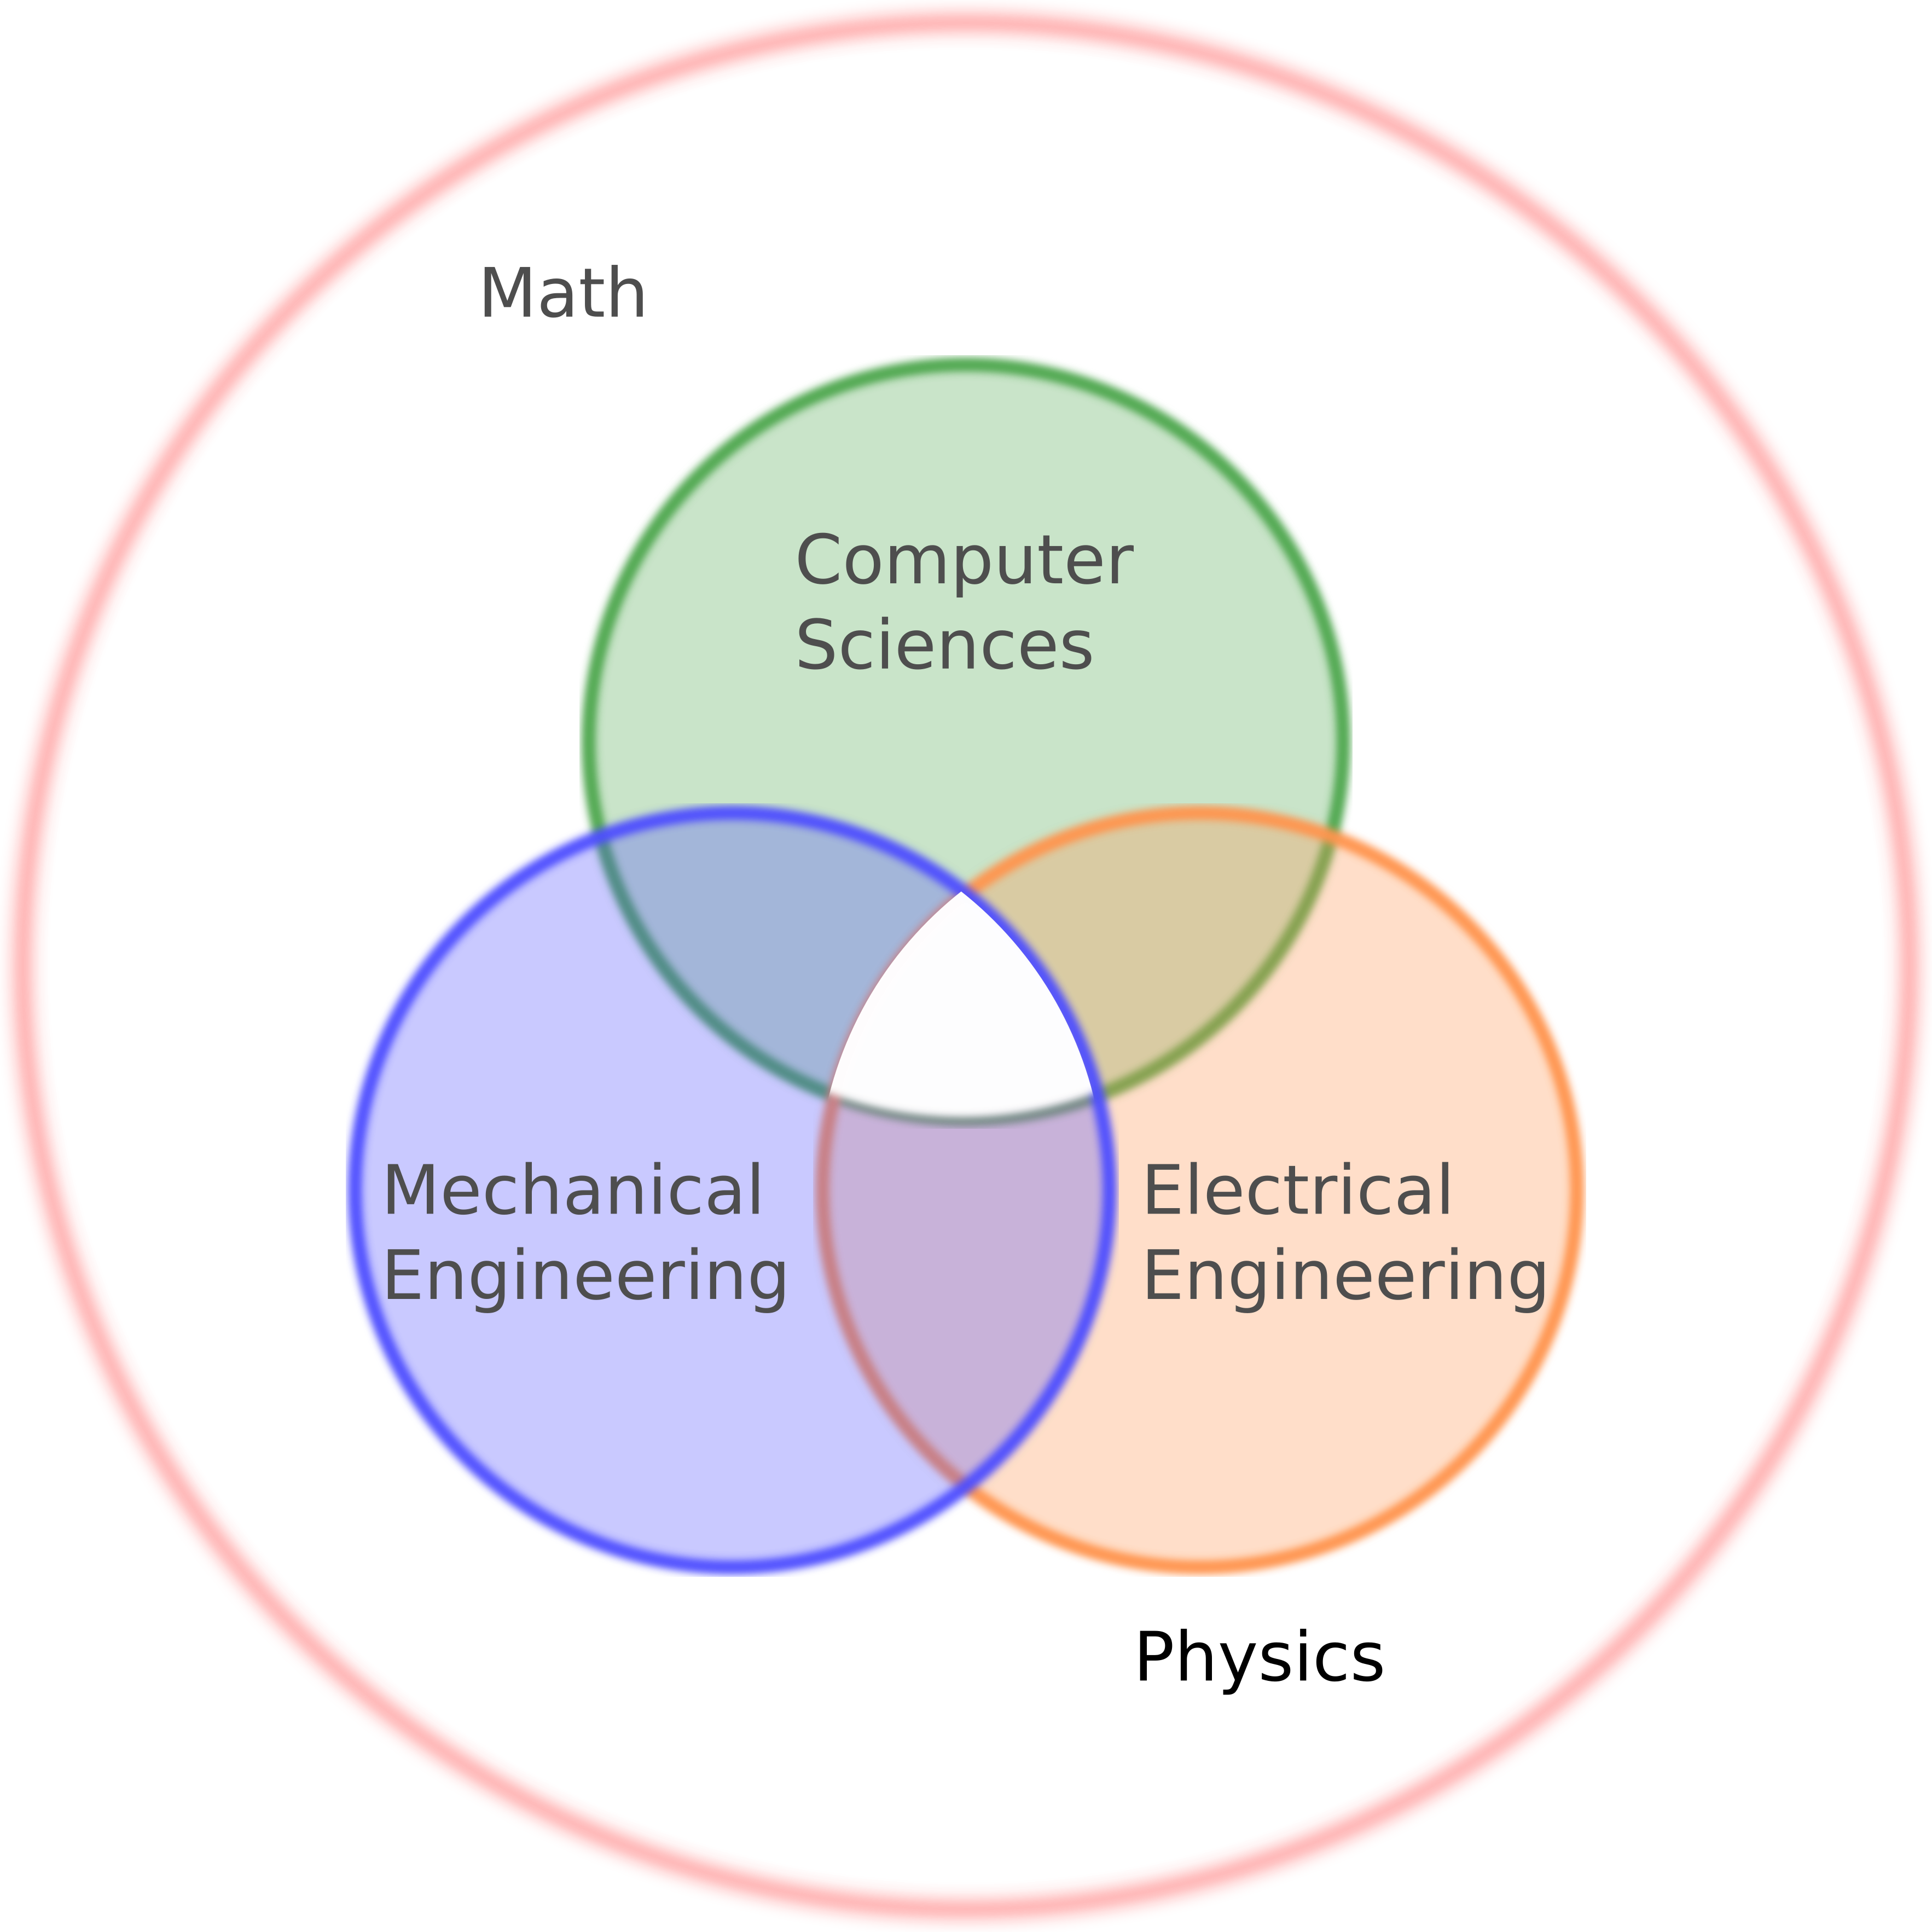
\includegraphics[width = 0.5\textwidth]{./pics/robotics_motivation.png}
    \end{figure}
  }

  % Show useage for simulation in context of mechanical engineering
  % Robot walking
  % Finite Elements
  % Path Finding
  % Mechatronics

  \frame{
    \frametitle{Simulation in the Context of Robotics}
    \begin{itemize}
    \item Structural Optimization
    \item Mechanical Prototyping
    \item Testing of Controller
    \item Learning
    \item ...
    \end{itemize}
  }

  % Show Targets for this lecture
  \frame{
    \frametitle{Lecture Targets}
    \begin{itemize}
      \item Basics: Modeling techniques
      \item Basics: System dynamics
      \item Basics: (Numerical) Stability of models
      \item Example : DC Motor
    \end{itemize}
  }


  \section{Modeling of Systems}

  \frame{
  \begin{figure}
    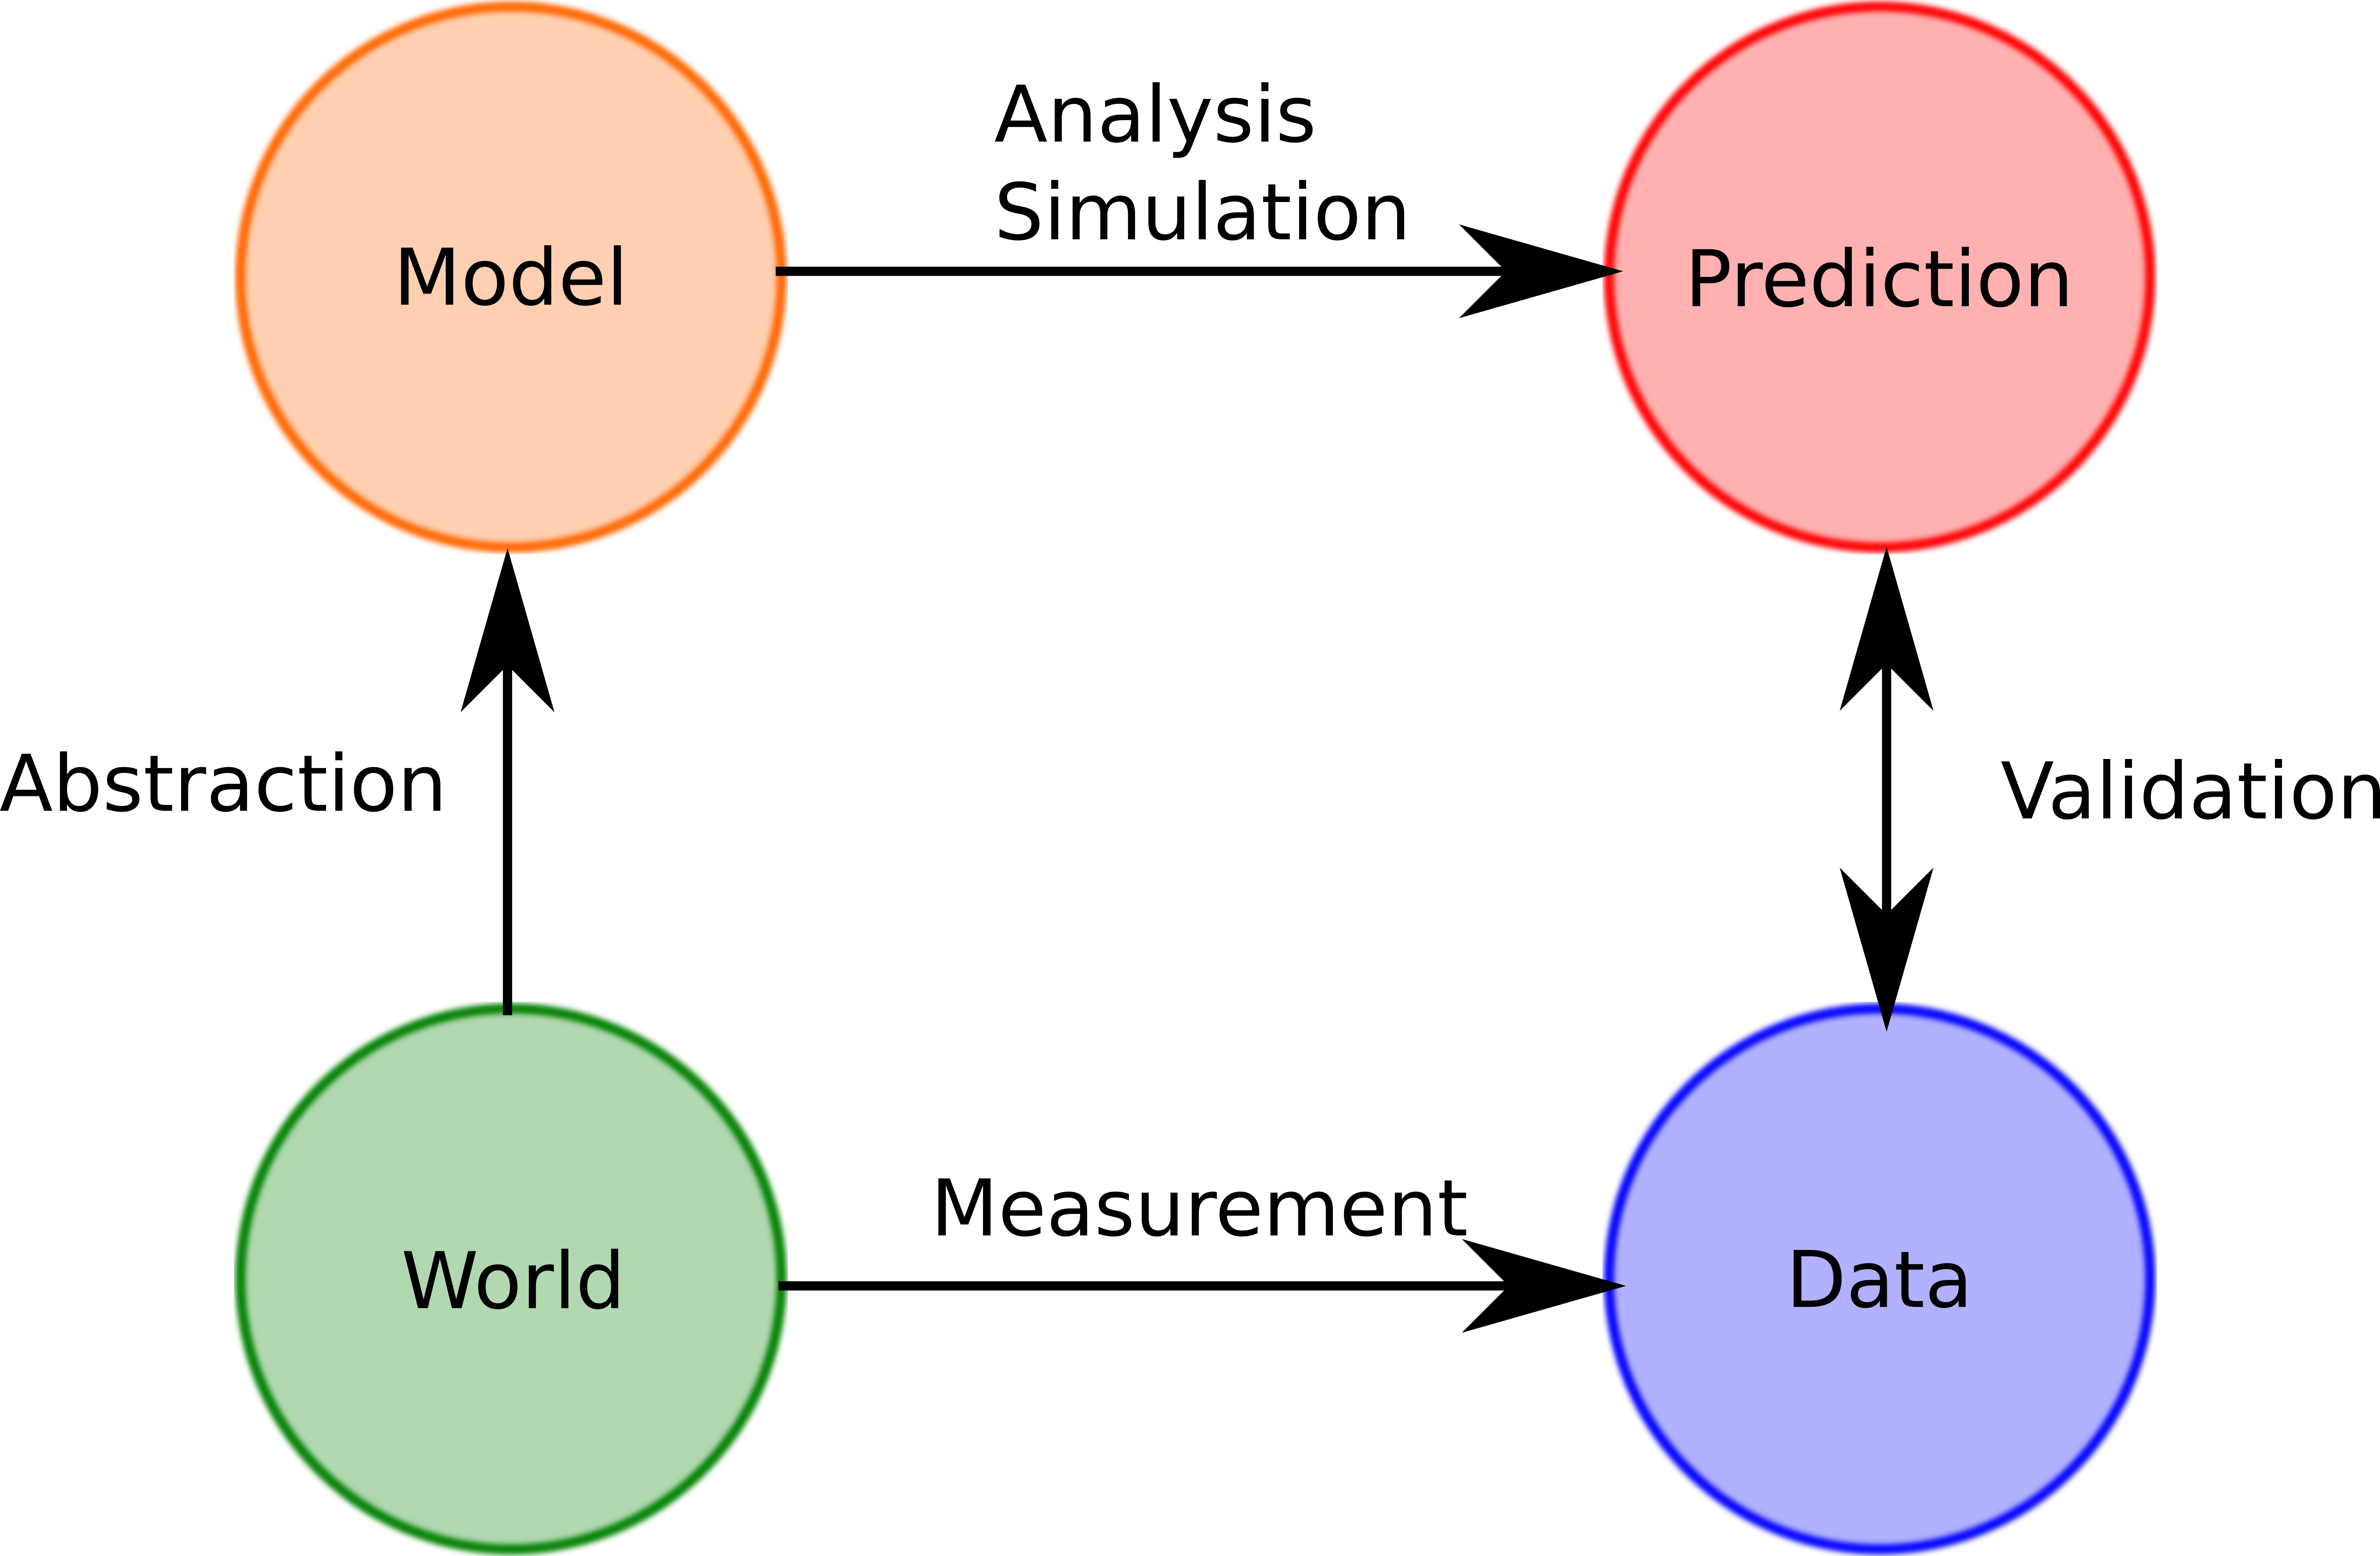
\includegraphics[width = 0.9\textwidth]{./pics/simulation_ideal.png}
  \end{figure}
  }

  \section{Basics of Systemdynamics}
    % Start with general system of ODEs
    \frame{

      % Initial Conditions
        \begin{exampleblock}<1->{Initial Conditions}
        The system at begin of our simulation or observation.
        \end{exampleblock}

      % Evolution
        \begin{alertblock}<2->{Evolution}
        The system propagates through time and changes.
        \end{alertblock}

      % Next State
        \begin{block}<3->{Next State}
        The system arrives at a new state.
        \end{block}
    }

    \frame{
    \begin{figure}
      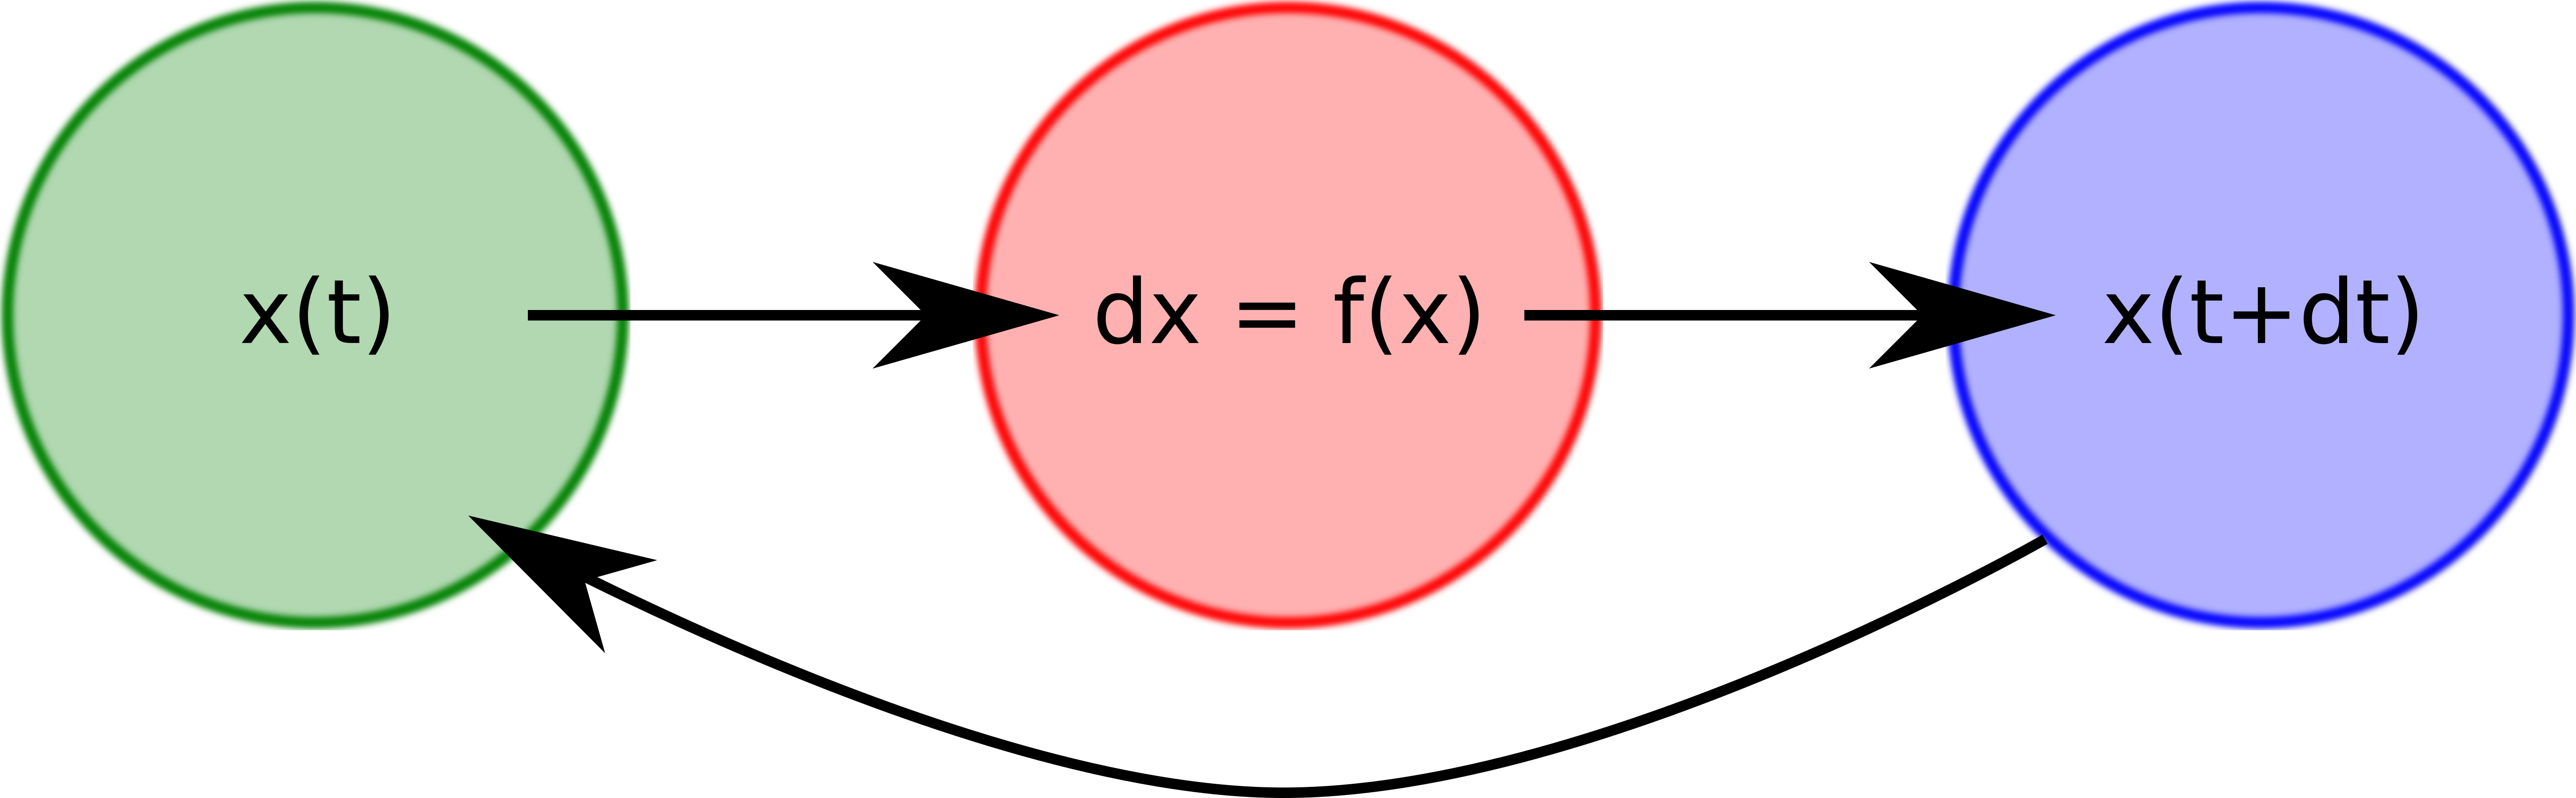
\includegraphics[width = 0.9\textwidth]{./pics/dynamics_concept.png}
    \end{figure}
    }

    \frame{
      In general, the system is given as a set of nonlinear differential equations.

      \begin{align*}
      \dot{x} &= f(x, u, t) \\
      y &= h(x,u, t)
      \end{align*}

      Where $x \in \mathbb{R}^{n_x}$ is called the state , $u \in \mathbb{R}^{n_u}$ the inputs
      and $y \in \mathbb{R}^{n_y}$ the outputs of a system. \newline
      The function $f : \mathbb{R}^{n_x} \times \mathbb{R}^{n_u} \mapsto \mathbb{R}^{n_x}$ evolves the system through time while
      $g : \mathbb{R}^{n_x} \times \mathbb{R}^{n_u} \mapsto \mathbb{R}^{n_y}$ defines the output.
    }



    % Reduce to linear equations
    \frame{
      For many systems a set of of linear differential equations is sufficient

      \begin{align*}
      \dot{x} &= Ax + Bu\\
      y &= Cx + Du
      \end{align*}

      With the state matrix $A \in \mathbb{R}^{n_x \times n_x}$, the input matrix $B \in \mathbb{R}^{n_x \times n_u}$,
      the output matrix $C \in \mathbb{R}^{n_y \times n_x}$ and the feedthrough matrix $D \in \mathbb{R}^{n_y \times n_u}$
    }

    \frame{
    \begin{figure}
      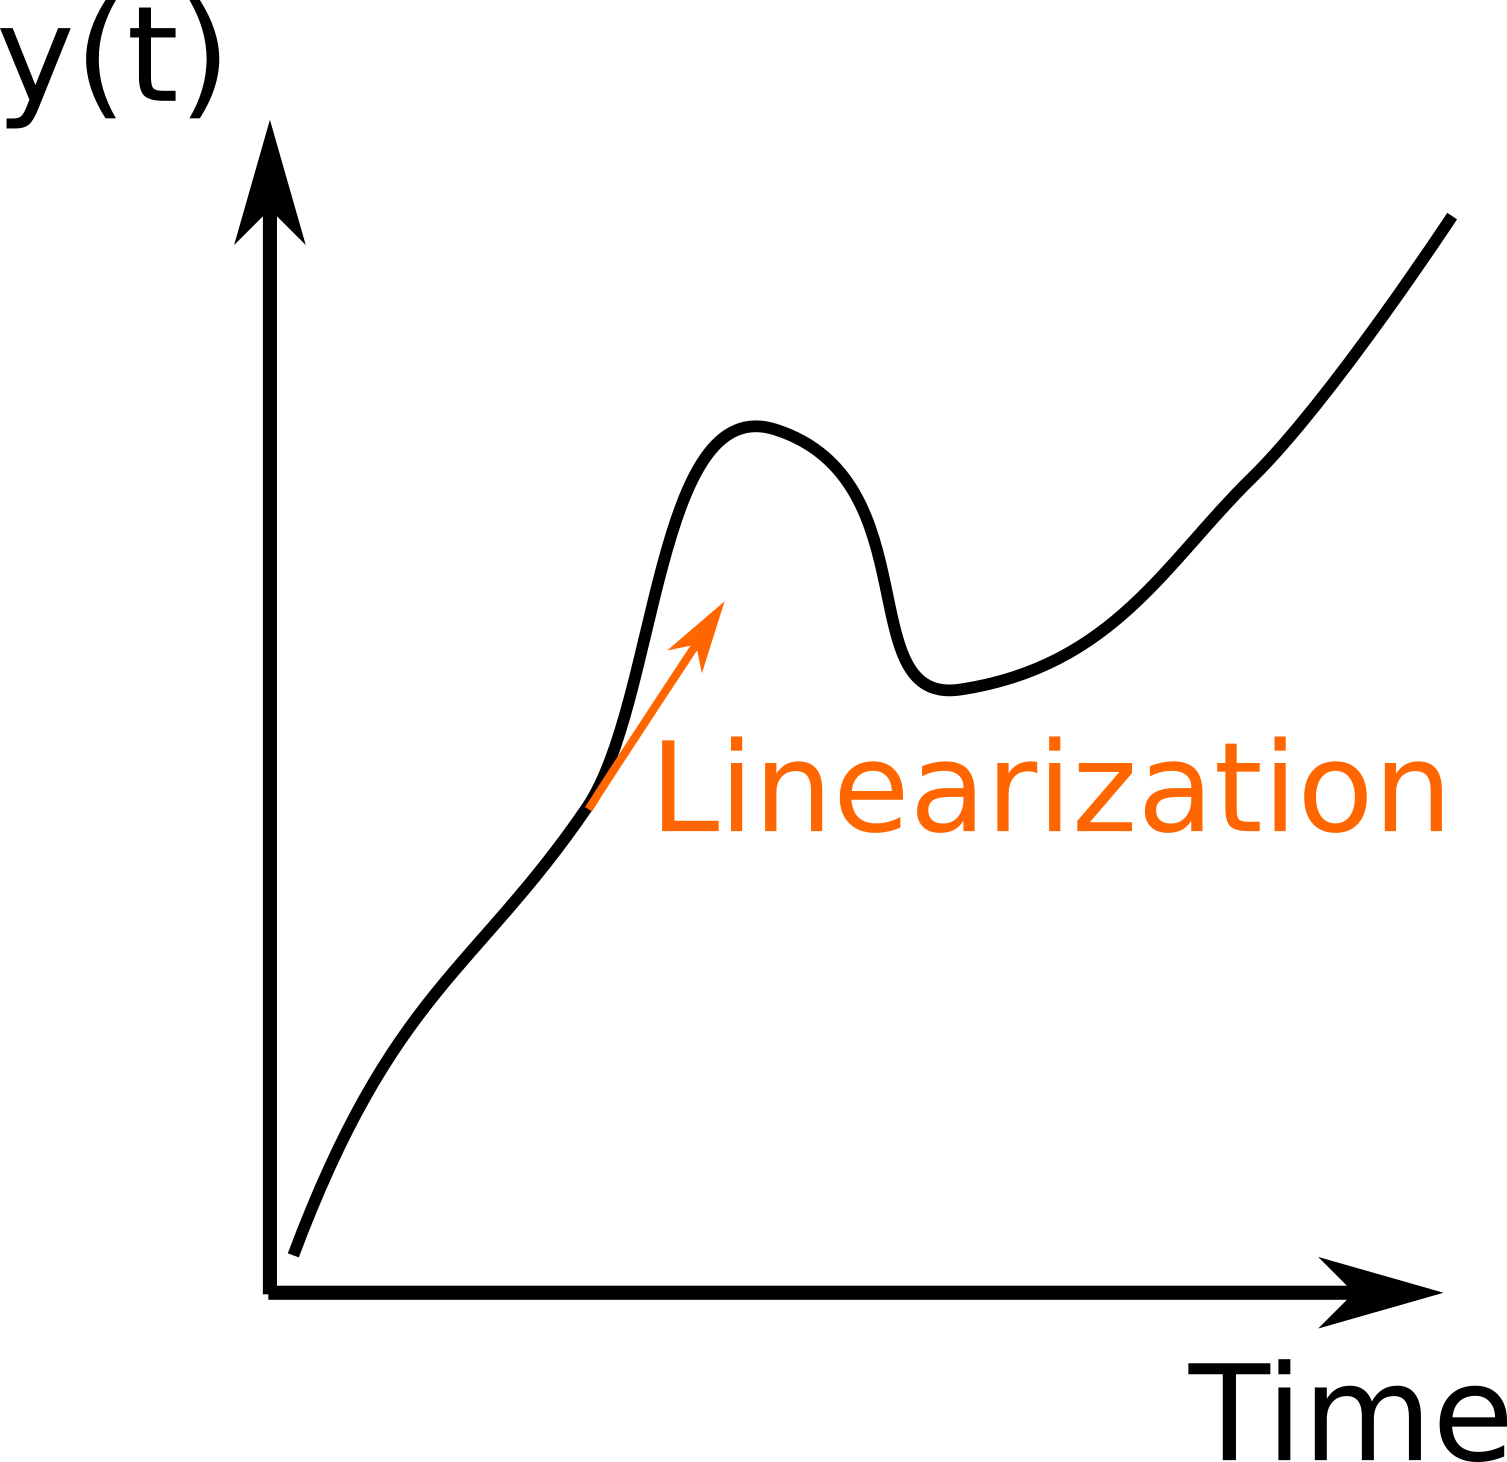
\includegraphics[width = 0.5\textwidth]{./pics/linearization.png}
    \end{figure}
    }

    % Example: Pendulum

    \frame{
      \frametitle{Pendulum}
      % Whiteboard : Derive EQM
      \begin{column}{0.5\textwidth}
      \begin{figure}
        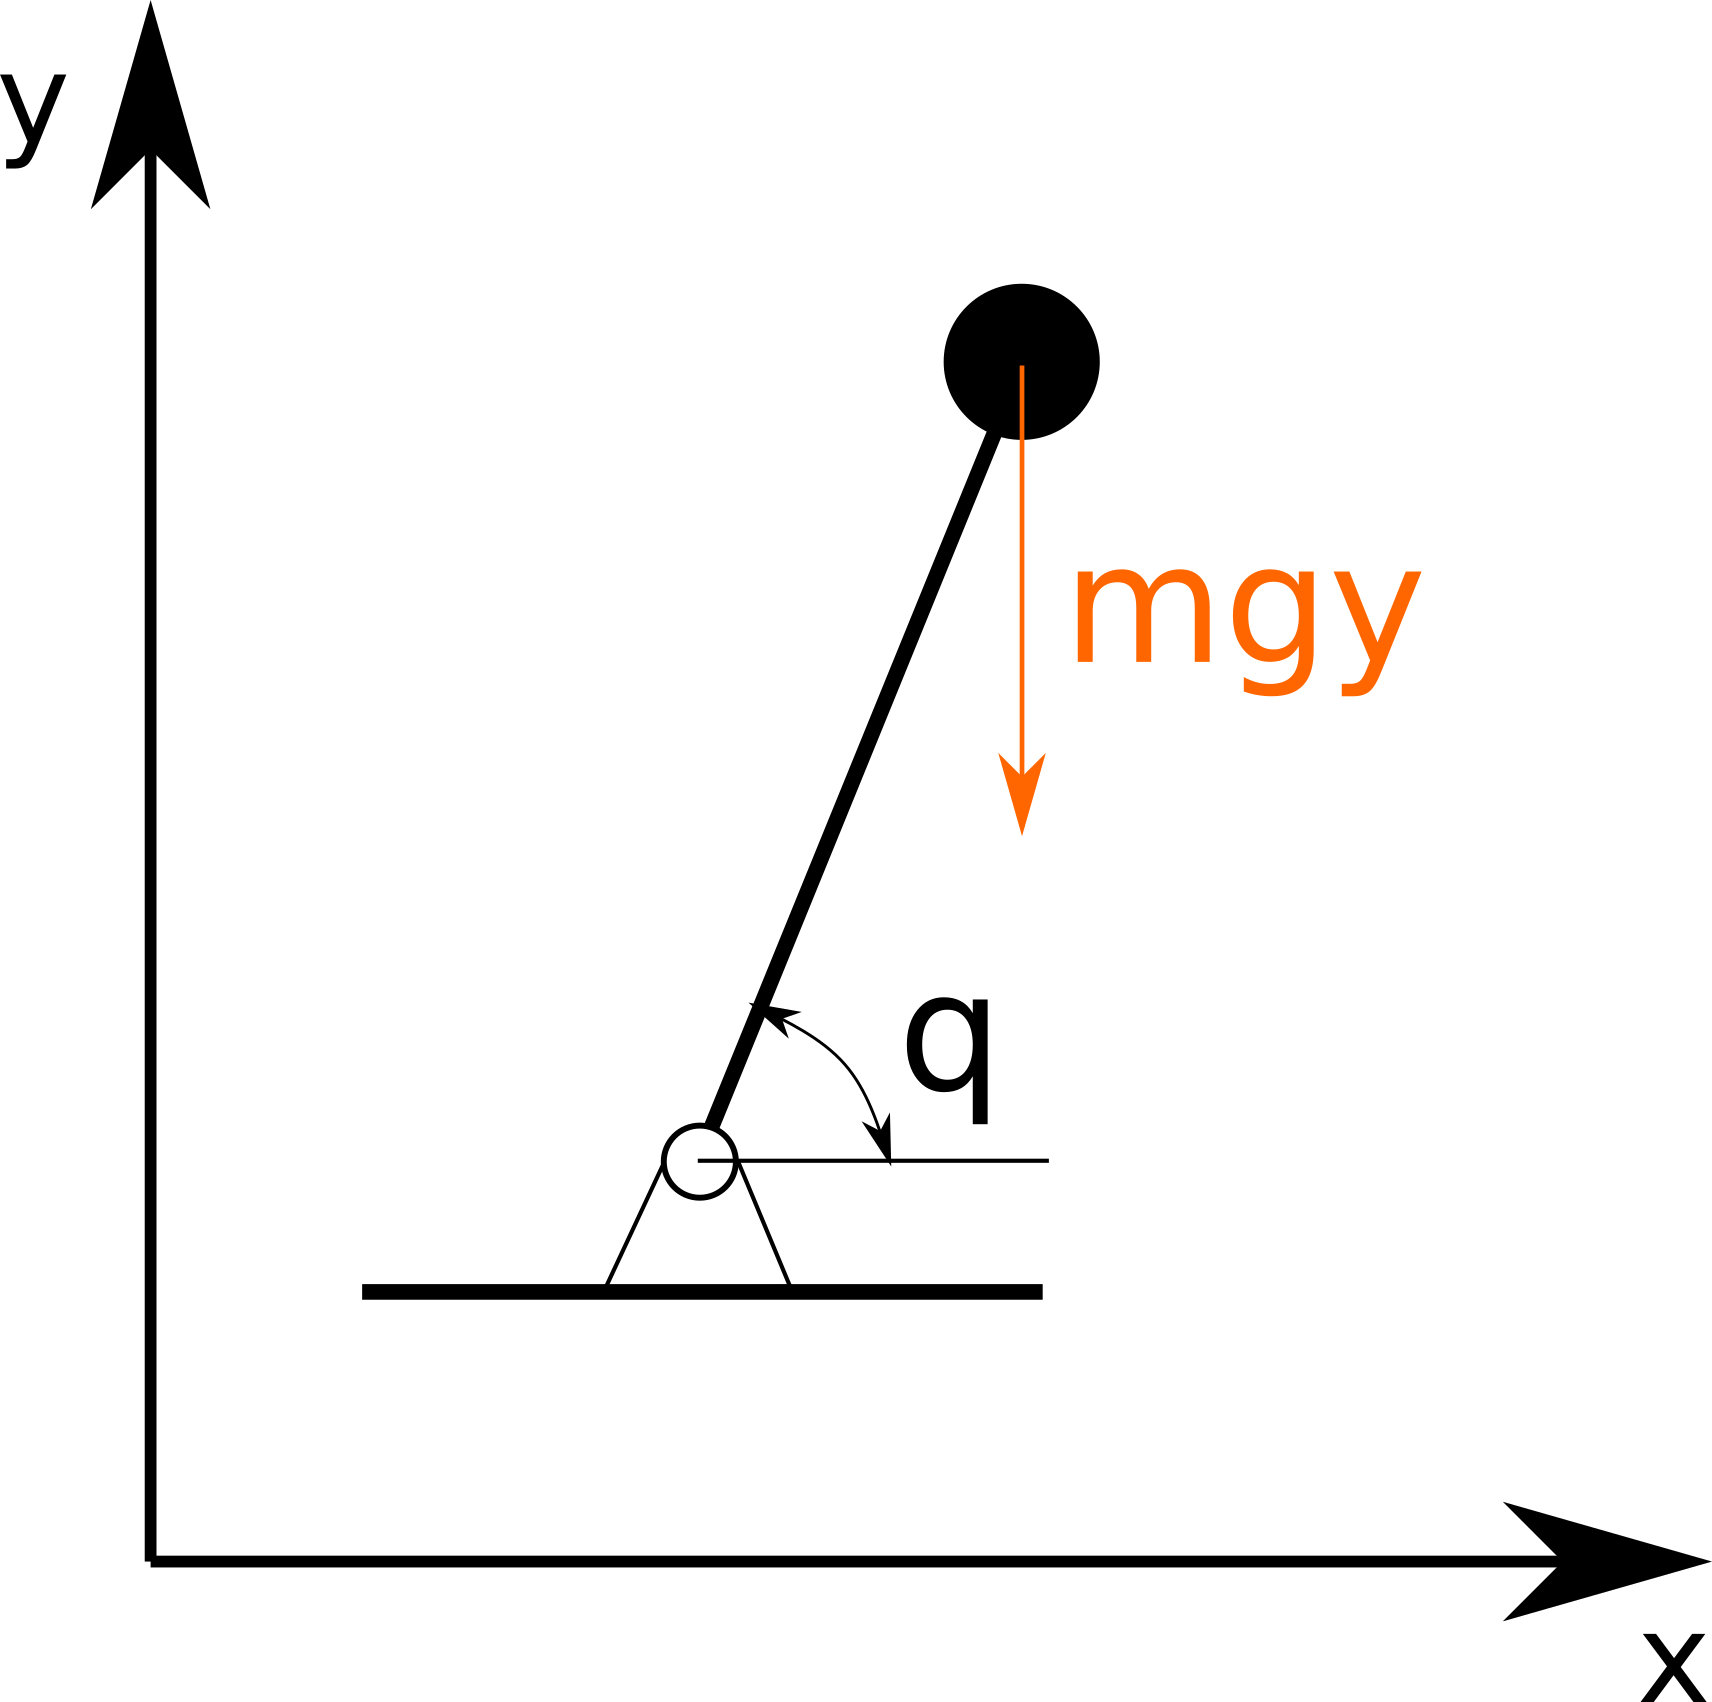
\includegraphics[width = 0.5\textwidth]{./pics/pendulum.png}
      \end{figure}%

      \begin{align*}
        \dot{\phi} &= \frac{p}{l^2 m} \\
        \dot{p} &= mgl~cos(\phi)
      \end{align*}

      \end{column}%
      \begin{column}{0.5\textwidth}
      Phase portrait
      \end{column}
    }


  \section{Stability of Simulation}

    \frame{
    \begin{column}{0.5\textwidth}

      \begin{exampleblock}{Status}<1->
        Continoous model in form of a system of (nonlinear) equations.
        \end{exampleblock}

        \begin{block}{Task}<2->
        Simulate the system over time
        \end{block}

        \begin{alertblock}{Problem}<3->
        Discrete calculation!
        \end{alertblock}
      \end{column}%
      \begin{column}{0.5\textwidth}

        \begin{align*}
        \dot{x} &= f(x, u) \\
        y &= g(x,u) \\
        \downarrow \\
        x_{i+1} &= F(x_i,u_i) \\
        y_{i+1} &= G(x_i, u_i)
        \end{align*}

      \end{column}
    }

    \frame{
    \frametitle{Example : Forward Euler Scheme}
      \begin{column}{0.5\textwidth}
      \begin{align*}
        \dot{x} &=  f(x,u) \\
        &\approx \frac{x_{i+1} - x_i}{\delta t} \\
        &= f(x_i, u_i) \\
      x_{i+1} &= x_i + \delta t ~f(x_i, u_i)
      \end{align}
      \end{column}%
      \begin{column}{0.5\textwidth}
      \begin{figure}
        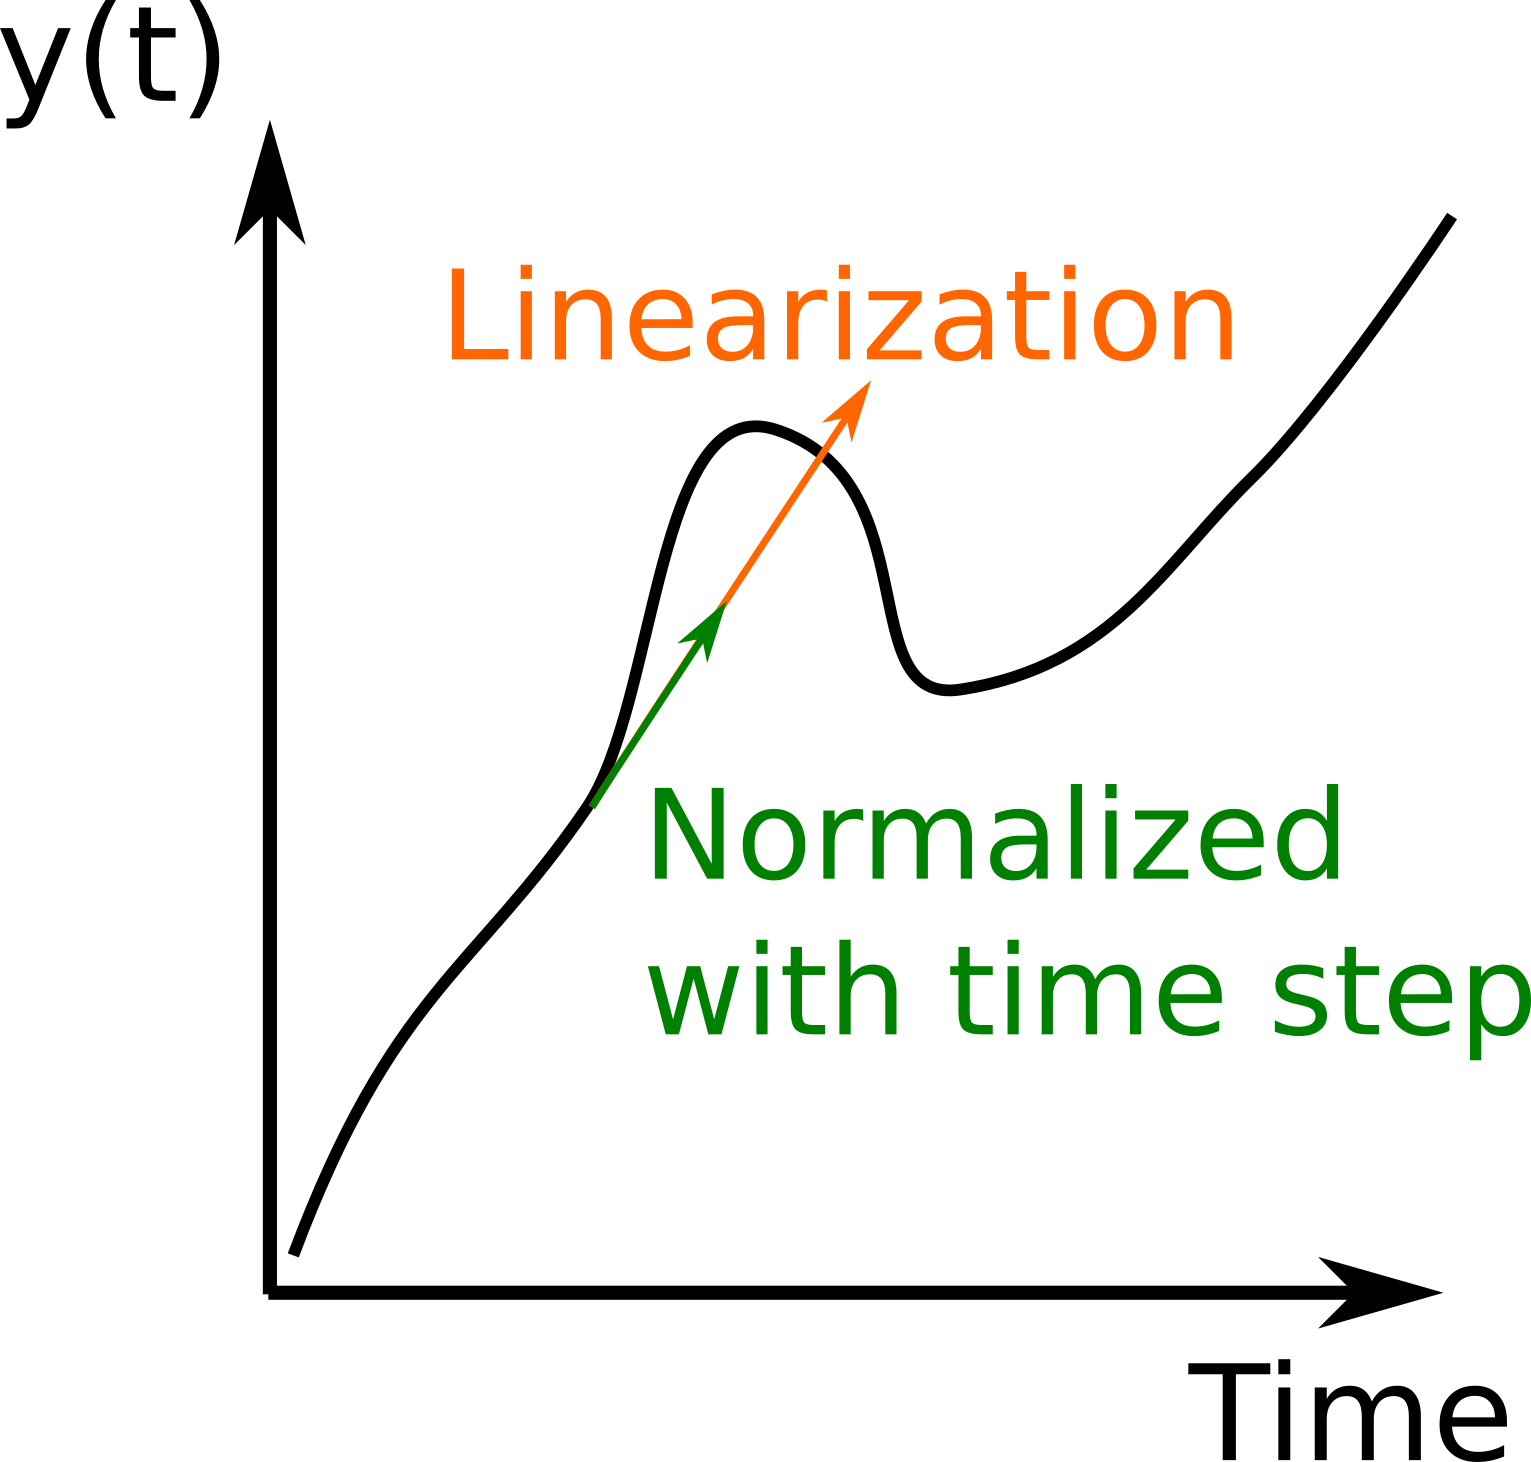
\includegraphics[width = 0.8\textwidth]{./pics/linearization_stepsize.png}
      \end{figure}

      \end{column}
    }

    \frame{
      A system is stable if trajectories starting near a final state end in this state or enter a closed orbit in its neighborhood.

      \begin{column}{0.5\textwidth}
      \begin{align*}
        x_S &= \{x \in \mathbb{R}^{n_X} | f(x_S) = 0 \} \\
        x_S &= \{x \in \mathbb{R}^{n_X} | f(x_S) \leq \epsilon \}
      \end{align*}
      \end{column}%
      \begin{column}{0.5\textwidth}

      Image - Stability on Phase space
      \end{column}
    }

    \frame{
      \frametitle{Stability - Direct Method of Lyapunov}
      \begin{column}{0.5\textwidth}
      A given system is stable of the form
      \begin{align*}
        \dot{x} &= -A x
      \end{align*}
      is stable if all eigenvalues $\lambda_i$ are on the right half plane of the complex plane.
      \end{column}%
      \begin{column}{0.5\textwidth}
      \begin{figure}
        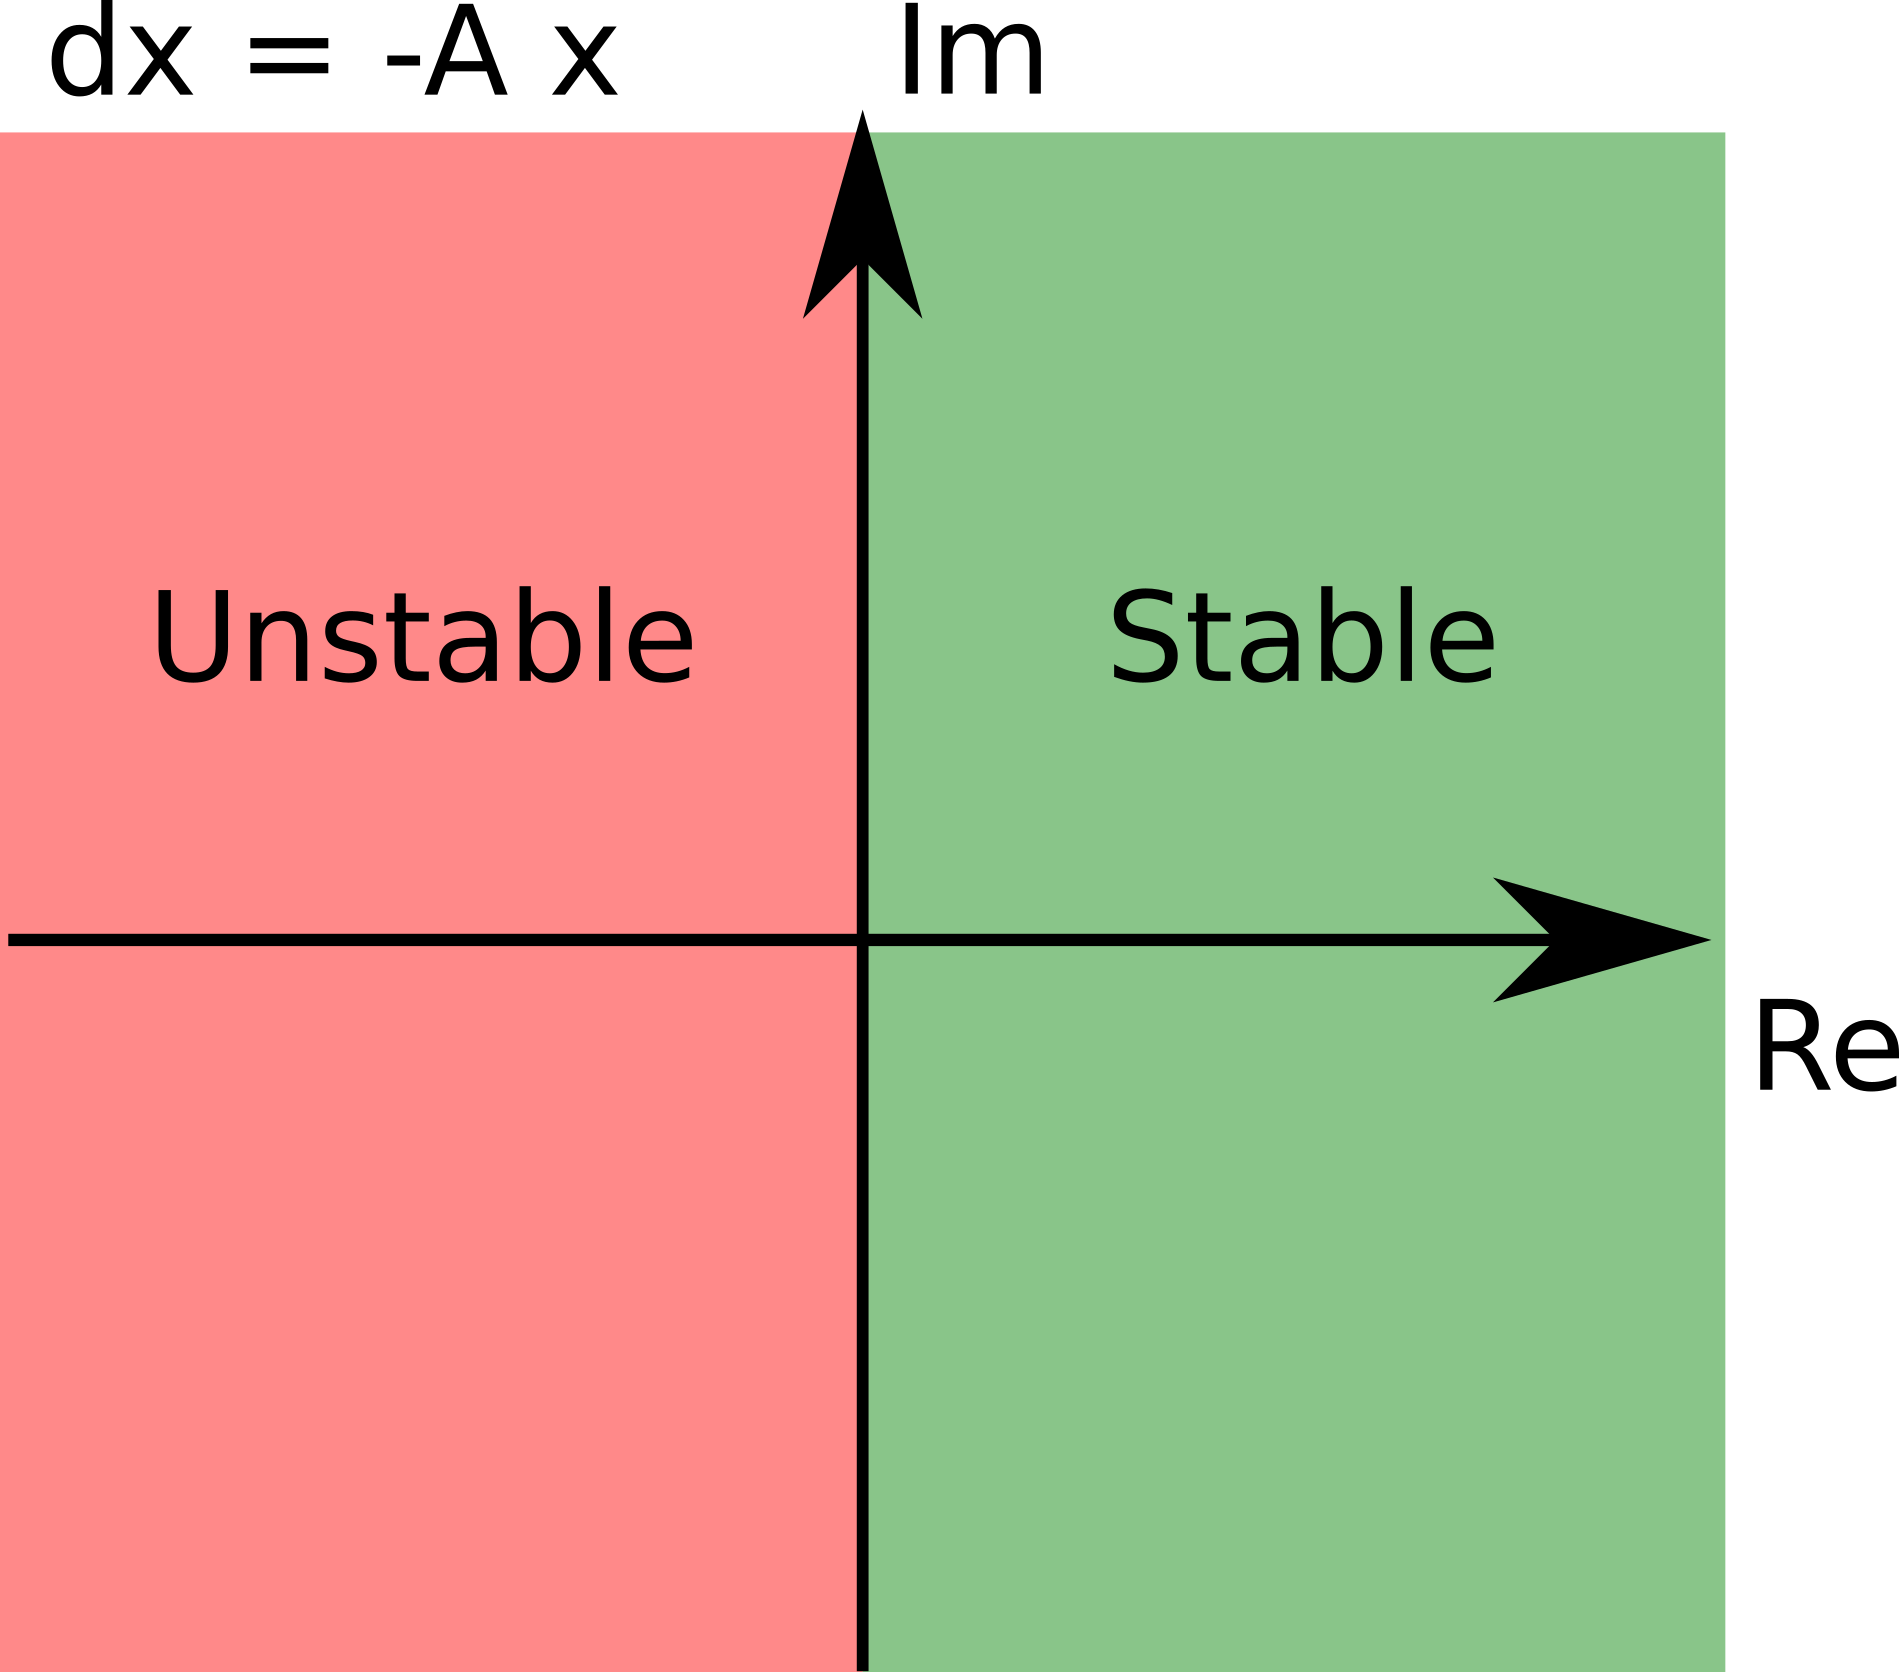
\includegraphics[width = 0.8\textwidth]{./pics/stability.png}
      \end{figure}
      \end{column}
    }

    \frame{
      Most physical system derived by first principles are stable due to conservation laws! \newline

      However, instability is possible due to wrong parametrization, the solver or the nature of the problem itself ( stiffness of differential equations).

      \begin{figure}
        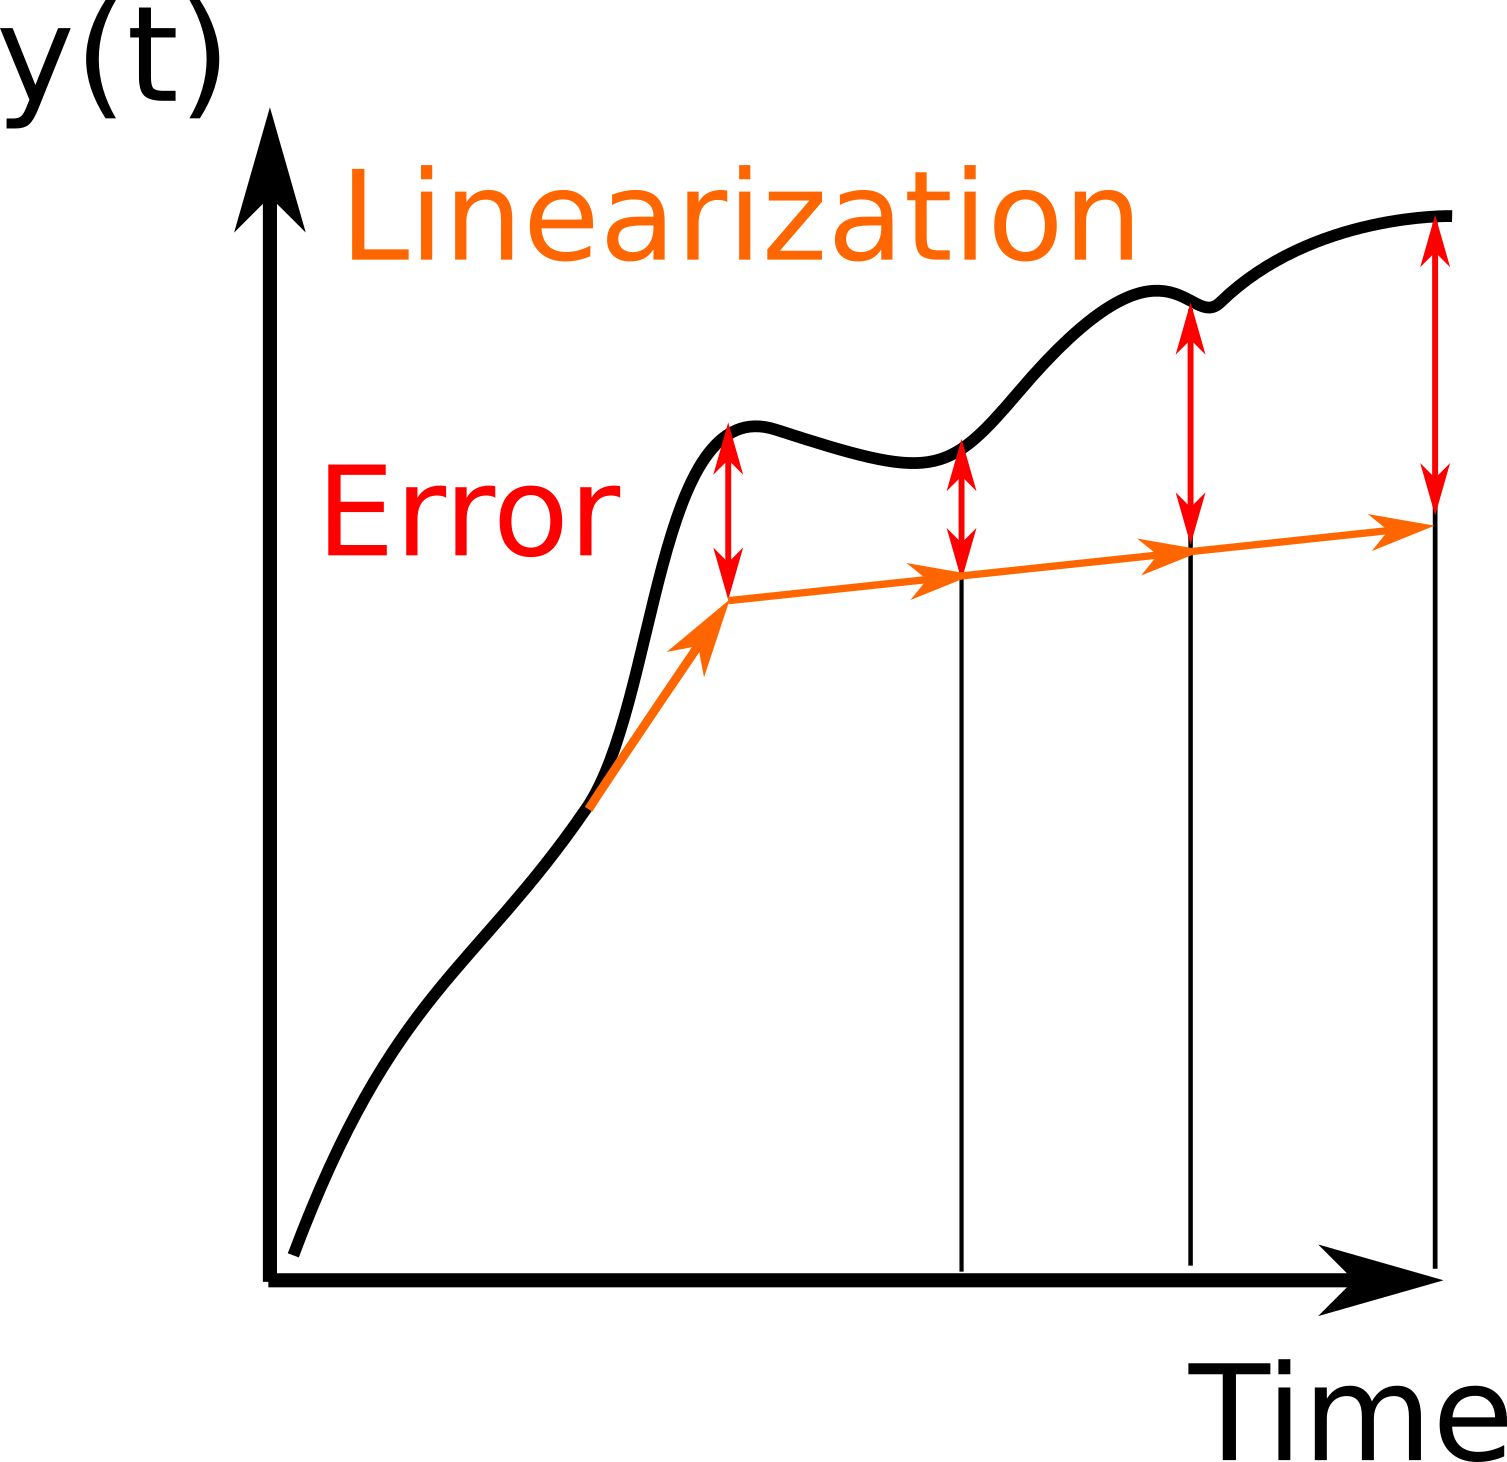
\includegraphics[width = 0.3\textwidth]{./pics/linearization_error.png}
      \end{figure}

      An stability criterion for numerical solver is the asymptotic stability.
      % Steifigkeit : Condition no of the transition matrix
      % Solver : Error Propagation due to solver
      % parametrization : Step size, convergence limit etc.
    }



    \frame{
      \frametitle{A-Stability}
      A solver is called asymptotic stable, if for a given problem of the form:
      \begin{align*}
        \dot{x} &= -A x, ~ Re(\lambda_i(A)) > 0
      \end{align*}
      The resulting calculation is monotonic decreasing for $\forall \delta t \in \mathbb{R}^+$
    }

    \frame{
      Consider the Pendulum in Euler Forward Notation:

      \begin{align*}
      x_{i+1} &= \begin{bmatrix} \phi_i \\ p_i \end{bmatrix} + \delta t \begin{bmatrix} \frac{p_i}{l^2 m} \\ m*g*l*cos(\phi_i)\end{bmatrix} \\
      &= \left[ I + \delta t ~\begin{bmatrix} 0 & \frac{1}{l^2 m} \\ mglsin(\phi_i) & 0 \end{bmatrix}\right] \begin{bmatrix} \phi_i \\ p_i \end{bmatrix} + \mathcal{O}^2
      \end{align*}

      The eigenvalues are then given as:
      \begin{align*}
      \lambda_i &= 1 \pm \delta t \sqrt{\frac{g}{l}sin(\phi_i)}
      \end{align*}

      Hence, the system is not alway stable, both in the sense of the step size or the formulation.

    }

    \frame{
      Stiffness of the problem:

      \begin{align*}
      \mu &= \frac{max(Re(\lambda_i))}{min(Re(\lambda_i))} \\
          &= \frac{1 + \delta t~\sqrt{\frac{g}{l} sin(\phi_i)}}{1 - \delta t~\sqrt{\frac{g}{l} sin(\phi_i)}}
      \end{align*}
    }

    \frame{
      Abschluss, wdhl
    }
  \section{Example: Modeling a DC Motor}

  \frame{
    \frametitle{A simple DC Motor}
    Bild
    % Aufgabe: Welche Dinge sind hier wichtig
    % Welche Parameter
    % Welche Gleichungen führen zur DGL?
    % Herleitung am Whiteboard
  }

  \frame{
    % Notizseite für DGL
  }


\end{document}
